\documentclass[25pt, a4paper]{article}
\usepackage{graphicx}
\usepackage[margin = 1.25 in]{geometry}
\usepackage{wrapfig}

\begin{document}
\title{CHAPTER VIII \\ BALKAR AND BEZINGI}
\maketitle	
\begin{flushright}
		\textit{Cold, insipid, smouchy Tartars.\\ CHARLS LAMB}
\end{flushright}
\begin{wrapfigure}{l}{0.4\textwidth}
	\centering
	\vspace{-40pt}
	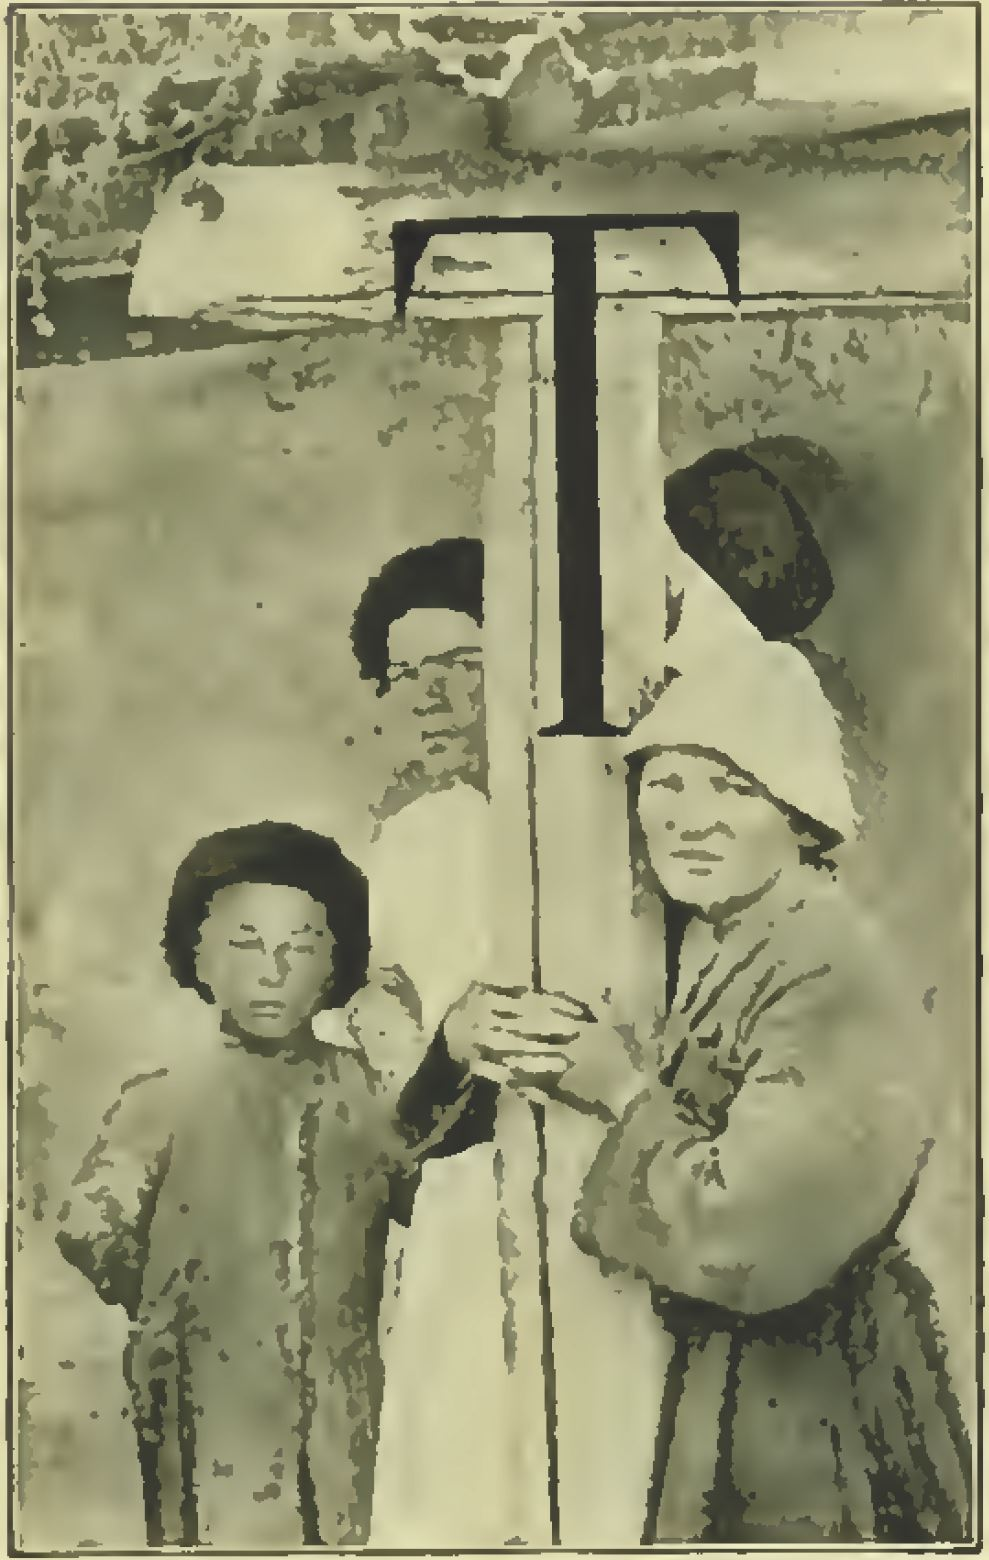
\includegraphics[width=1\linewidth]{Figure 1}
	\vspace{-30pt}
\end{wrapfigure}
\paragraph{} \normalsize The limits of the Central Group, the heart of the Caucasus, have been defined, very conveniently by Nature. The geologist as well as the topographer finds a clear boundary laid down for him. The granite stretches from the Agashtan Pass westward to the Zanner; on both these tracks the traveller finds crumbling slopes of crystalline schists. The Central Group comprises the main chain from Fytnargyn to Gestola, with the great spur which circles horse-shoe-wise round the Mishirgi Glacier and includes Dykhtau and Koshtantau
	
\paragraph{} In 1868 nobody knew anything about these mountains, except that two of them had been measured and called Koshtantau and Dykhtau by the Russian Surveyors. The first English mountain explorers were puzzled, and we naturally made some serious mistakes. So did Mr. Craufurd Grove and Mr. Clinton Dent, who followed us. The Koshtantau of the old five-verst map (now called Dykhtau) we identified with Shkara; our successors confused Gestola with Tetnuld. It was not until 1887 that I was able to show positively that the gigantic Shkara had been ignored by the earlier survey and that Mr. Dent's “Guluku” was the five-verst Koshtantau, since renamed Dykhtau. Slowly we worked out the nomenclature and topography with the imperfect means at our disposal. Mr. Donkin's map, published in the Alpine Journal for 1888, was the first-fruits of the revival of interest in the Caucasus; my map in the Proceedings of the Royal Geographical Society followed it at a year's interval. Soon afterwards the results of the new one-verst survey began to come in and we found in many districts our preliminary investigations corroborated, extended, and made more precise, by the work of a government staff. It is only fair, however, to point out that several of the sheets of the new map, printed—the Elbruz sheet alone has yet been published—before the Surveyors and Alpine explorers came into close and friendly contact, were far from correct in the upper regions. The Austrian map of Tyrol had to be revised in accordance with the knowledge of mountaineers. Without the example of Mr. Adains Reilly, the French map of Mont Blanc might have been no better than other mountain portions of the contemporary survey. It is no discredit to the Caucasian Staff if it has to some extent profited by similar communications.
	
\paragraph{} In my first visit in 1868 to the Central Group we climbed no snowy heights. Nor were Mr. Craufurd Grove and his companions more successful in 1874. To that expedition the public owes a work which has long been scarce, and deserves to be reprinted. The Frosty Caucasus is a lively and at the same time very accurate series of sketches of Caucasian travel and Caucasian people. But, though it includes the story of the first ascent of the highest peak of Elbruz, it is in the main a record rather of travel than of climbing. It is possibly on this account that it has proved so generally attractive. There is, it must be confessed, a certain monotony in the innumerable pages in which we Jacks and Jills of the day record our experiences on uneven ground.
	
\paragraph{} In the preceding chapters the traveler has been brought from the east to the foot of the great peaks. The man in a hurry —the traveler who has only six weeks to give to the Caucasus —will probably wish to go straight to its most characteristic scenery, to Karaul, the Bezingi Glacier, Chegem, and Suanetia. Should he come from the south by way of Batum and Kutais, he will cross one of the Rion passes. This plan has advantages, as he can easily dispatch provision cases from Kutais to Suanetia to meet him. But should he land at Novorossisk, and take the Caucasian Railway, Naltshik is his nearest starting-point for the mountains.
	
	At Kotlarevski, a station or two beyond the Mineral Baths, he will see the daily train with its luxurious cars disappear into the distance, while he is left surrounded by a heap of the more or less shapeless boxes and bundles that a Caucasian tour necessitates. The station itself is not much behind a country station in England. Tea may be had, or red water-melons and loaves of Russian bread; there are leathern sofas in a waiting-room. But at its door the luxuries of travel end. The post-road to Naltshik, an important administrative center, is the part of the steppe where carriages pass. The vehicles are not the commodious tarantasses or phaetons of civilized Russia, but the cruel carts called telegas, shaped like broken-down tub-boats, and set upon wheels with no intervening springs. The steppe, however, is less stony than the wilds of Armenia, and six hours of slow jolting, during which, in clear weather, the view of Elbruz is some consolation to the mountaineer, will bring him and his baggage to the gates of Naltshik.
	
	Perhaps Naltshik has no longer a gate. On my first visit it certainly boasted of a wooden barrier, guarded by a sentry, while a stockade surrounded the settlement. Under the influence of less troublous times the old military cantonment has developed into a quiet country town. The broad streets or roads are shaded by trees and bordered by one-storied, paint-brightened, green-roofed cottages or bungalows, each standing detached in its own garden plot. There are several stores, where the Russian or German colonists supply their wants, or the hill-men purchase such simple implements or luxuries as they can afford. The local architecture might remind the traveler of rural Holland, were it possible to imagine an untidy Holland.
	
	As an administrative center Naltshik has considerable importance, for here lives the official, or Nachalnik, who is responsible for the peace of all the Turkish tribes between the Urukh and Elbruz, the men of Balkar and Bezingi, Chegem and Urusbieh. Heither the village chiefs, or Starshinas, come down to render a periodical account of their stewardship, to be instructed as to new forest regulations, or to discuss some moot point of
	
	rights of pasturage between their communities. Russian administration of Asiatic mountaineers, as far as a traveler sees it, is in many respects the opposite of our own m India. Contrast, for instance. Captain Younghusband's account of how we bewildered the folk of Gilgit at first by our activity, our demands for labor for public works, our insistence on public order. The Russian civil servant in the Caucasus, as a rule, does little he can help, unless it conduces to his own immediate amusement or advantage. The idea of developing his district, of adding to its natural resources, seldom seems to occur to him. The national talent for doing without roads naturally disinclines him to any efforts in their construction. I am afraid the national tendency to jobbery comes in also. No other explanation of the dozens of broken and useless bridges, the roads paid for by distance, which take a fatuously circuitous course, suggests itself to the Western mind, or has been offered to me by Russians themselves. On the other hand, if little is done for the mountain people of the Caucasus, comparatively little is required of them. They have never yet been systematically called on for military service, domestic disorders are easily overlooked, taxation is light, and in the mountains almost nominal. The Turkish tribes are not disaffected, but they might easily be persuaded to emigrate to some country whence the pilgrimage to Mecca would be made easier to them, and where they would feel less cut off from the Mohammedan world.
	
	It would be a pity. I trust that we may never hear of this fine race, so well suited to the highlands they inhabit, being driven, through misunderstanding with local officials on matters of administrative detail, to follow their Circassian neighbors in seeking a new home outside Russia, and thus to add a new element of disorder in lands where the nations of Europe, and England in particular, have too long supported that effete and barbarous system of extortion and misrule which is called the Turkish Government.
	
	The two main avenues of approach from Naltshik to the great glaciers at the sources of the Cherek are naturally the valleys of that torrent. Its two branches unite some miles above and to the east of the town, in a depression between the outer or cretaceous chain and the northern belt of limestones. To reach Bezingi a short cut over the lower hills is generally used. To Balkar the track strikes at once eastward to the Cherek, through a rolling country, the edge of the steppe, garnished with dogroses and wild fruit-trees, and but sparsely inhabited. This formed part of the Kabarda, so named after a race said to have come from the Crimea, who made themselves masters of this part of Circassia. The villages are long ranges of simple wooden huts or sheds, and gardens surrounded by wattled fences. They lie in the open country. The hills and woods are the old debatable ground, and no human habitation except a shepherd's hut is met during a long day's journey and till after the great limestone gorges have been left behind. In 1868 we rode up from Naltshik to Balkar in two days. A Cossack will reach Karaul in the same time: but mountaineers new to Eastern travel may find the days long enough; for Turkish saddles, if difficult to be thrown out of, are irksome to remain in—though habit may do much.
	
	After the river has been crossed the forest becomes beautiful enough to call forth enthusiasm, even from those who are no novices in the Caucasus. Crags jut out from the green slopes and afford a home to delicate ferns; moss-cradled brooks pour down out of secret hollows. The tall smooth trunks of elm and alder are festooned with the long streamers of creeping plants, the common rhododendron and golden azalea grow to an immense size. A tarn, fringed with grasses, reflects on its surface the overhanging crags and boughs, and suggests a mid-day halt. We camped not far off in 1868. In 1847, this neighborhood was the scene of a more imposing encampment. The famous Schamyl, the leader of the tribes of Dagestan, penetrated to this point in an attempt to raise the Central Caucasus, having with him a formidable host of Chechens and six cannon. His immediate object was to establish himself in the basin of Balkar and hold it as a citadel whence he might sally forth into the Kabarda, the inhabitants of which would, he hoped, make common cause with him. But the Tauli, or Mountain Turks, in place of welcoming their co-religionists, barricaded the great gorge against them; the flocks sent from the Kabarda were cut off by the Cossacks, and one night the armed host suddenly struck camp and hurried back by forced marches to the forests of Chechnya beyond Vladikavkaz. It was a critical moment in the history of the Caucasus when the Moslem host, with its banners and its knights in chain armor, such a host as we read of in the tales of the Crusades, retreated to its native fastnesses; and the Russian Government owes no slight debt to the Balkar chiefs who prevented the flames of revolt smoldering on the shores of the Euxine from bursting into a blaze which would have spread from sea to sea.[1]
	
	The valley above our camping-ground was completely closed by precipitous limestone cliffs, which seemed to form a barrier against all further progress. The path—already at some height above the Cherek, glimpses of which could only be seen from time to time at the bottom of a deep ravine—turned abruptly upwards, and climbed rapidly through the forest. Having reached a height of at least 1500 feet above the bed of the river, it struck boldly into the heart of the gorge, circling round ravines, and winding over the top of the perpendicular cliffs, where a fall from one's horse on the off-side would have led to a short roll, followed by a sensational header of many hundred feet. The vegetation, wherever it could find room to cling on the shelves and crannies between the precipices, was magnificent ; pine and beech still predominated, though there was a sprinkling of other foliage. Single trees crowning some projecting crag, where, destitute of any apparent source of sustenance, they yet contrived to maintain a vigorous existence, added much to the beauty of the defile. Alpine flowers for the first time showed themselves in company with the most delicate ferns, and even the grandeur of the surrounding scenery did not make us forget to welcome such old friends.
	
	We could best appreciate the magnitude of the precipices immediately below us when a bend in the hillside enabled us to look back on some portion of the road already traversed; the cliffs on the opposite bank were even more tremendous. Half-way through the defile, a spur of the mountains on the eastern side of the river juts out straight across the gap, and in fact does at one spot actually touch the opposite mountain, leaving the water to burrow underground as best it may. The path descends on to the saddle connecting the rocky crown of this spur with the hillside from which it springs. This brow, from its position, commands a view both up and down the defile, to which there is nothing similar, or in the least comparable, in the Alps. The gorge of the Cherek is no mere crack in the lower slopes of the mountains, like those of Pfeffers and the Via Mala; it is rather a trench dug down from their very summits to a depth of 5000 feet or more. Behind us forest trees clung to every available inch of ground ; looking upwards, the character of the defile was more savage. The foaming waters of the Cherek. crossed three times by bridges, filled the bottom of the trench, the sides of which were perpendicular walls, succeeded by shelves capped in their turn by a loftier tier of precipices. The path, a mere ladder of broken stones, brought us by a rapid series of zig-zags to a most extraordinary spot, where the overhanging cliffs meet and form a natural bridge over the river, which can barely be seen at the bottom of its deep bed. Seen from this point, the torrent to all appearance plunged directly into the heart of the mountains, and it was impossible to discover how it found a way out. The savage grandeur of the scenery here attained its height, and so far as my own and my companions' experience goes, there is no gorge in the Central Caucasus of equal grandeur.
	
	Henceforth the cleverly contrived rock-staircase which connects Balkar with the outside world finds room—now on one side, now on the other—to creep along the base of the cliffs at the river's edge; until at last, just when the careless observer would think it was hopelessly defeated, it crawls across the face of an overhanging bluff by a gallery, partly cut into the rock, partly built out from it. We next wound over barren and disintegrated slopes, broken occasionally by stone-capped earth-pillars, similar to those we had seen before on the Ardon, in the Caucasus, and to the well-known examples in the Val d'Hérens in Switzerland.
	
	At last the difficulties are left behind, the cliffs draw back in two grand curtains, and the cultivated basin of Balkar, studded with human habitations, opens in front. A castellated farm or fortress watches the exit from the defile. The lower slopes—no longer cliffs, for we have passed from the zone of limestone to the crystalline schists—-are bright with corn; but not a tree is visible on the vast, monotonous green downs. The only incidents in the landscape are stone boundary-walls and stones in heaps or scattered. The heaps are villages, the scattered blocks mark graveyards.
	
	The people of these villages belong to a race numbering in all about 13,000 souls. They describe themselves as Mountain Turks, and claim to be a branch of the tribe who conquered Constantinople. In olden days they were ruled, in a more or less patriarchal manner, by chiefs whose authority was hereditary in the family and whose policy was directed by travelled Mullahs, who in their turn got their ideas from Istanbul or Mecca. Istanbul was their world's center; thither went adventurous youths, in the hope of ending their lives as pashas, and occasionally adventurous young women, not averse to becoming pashas' wives. Now these avenues for ambition are closed; orders have to be taken from Naltshik or Vladikavkaz, and the native appointed Starshina by the Government may exercise authority over the old village chief. Their home-life and occupations are little varied. They are rich in flocks and herds, cultivate much barley and brew an abominable substitute for beer, which an infatuated German (Klaproth), famous for his inaccuracies, once described as equal to the best London stout! One of their chief occupations is to collect brushwood for fuel, for which purpose they employ innumerable donkeys. They hire southerners, Mingrelians or Suanetians, who come in crowds across the glacier-passes to mow their hay-crop and for other labour, while they themselves enjoy sport and society after the manner of the country. Capital walkers, keen hunters, they are still keener conversationalists. Subjects for conversation being naturally limited, they make the most of what material they have. Their legends extend from Prometheus to the first climbers of Elbruz. If travelers’ tales are not always exact, tales about travellers never are—at least according to my experience. I am said—so it has been reported to me—to have paid some Suanetians 80 roubles to declare I had ascended Ushba. I did pay this sum—for porterage in 1868 at Urusbioli. The disappearance of Mr. Donkin's party in 1888 was naturally a subject for much invention, and the German interpreter who was with the mountain-climbers was, I believe, made the subject of many quite groundless calumnies. Clubs and newspapers are still unknown to these secluded mountaineers: they leave to manufacture their own gossip, and—like their beer—it is but an inferior article. 
	
	
	
	
	I have already described an Ossete village. The Turkish villages are of the same type, only while the Ossete house is more of a building, the Turkish is more of a burrow. The timber of which the roofs and porticos are made, axe-cut without the aid of a saw, is more massive ; the windows are even smaller ; they have no glass, only wooden shuttei's ; the greater part of the house is dug out of the hillside, so that the flat i-oof hardly interrupts noticeably the general slope. A great field of the dead, thickly planted with immemorial tombstones, surrounds the houses of the living. The tombstones are rough blocks, or in the case of men of note tall slabs, sometimes capped by a stone turban or covered with inscriptions, sometimes engraved with representations of the horse and accoutrements of the deceased. Thus is preserved the memory of the earlier time, when the horse was slaughtered and the arms buried for their owner's use in another, but not a better, world. The Mosques may easily escajse notice. Except at Chegem, where one has been designed under external influences, they are low large halls, without architectural ornament, and it is from a houseroof or low platform and not from a minaret that the Muezzin's voice wakes the echoes of the hills.
	
	As our cavalcade files along the muddy lane that serves as a street the roofs are crowded with women, clad in loose, red robes, with rows of coins hanging from their caps, over which and their faces they forget, in the unwonted novelty of the event, to draw their veils. In the doorway gather companies of tall, bearded, grey-frocked men, with daggers and pistols at their belts and swords dangling from their girdles. One, taller than the rest, in an overcoat of inverted sheepskins, steps forward and salutes the interpreter. He is the Starshina, or village chief, responsible to the Government for the peace of the district. In the old days he received strangers in his guest-house ; now they are sometimes invited to find lodging in the generally bare and mouldy room of a so-called Cancellaria or court-house. They may often do better for themselves by making inquiries for the storekeeper of the valley, the man of enterprise, who, with a painful disregard of local colour, has put a tin roof and a boarded floor to his house, and keeps a small store Avith the goods he fetches up once in three months from Naltshik.
	
	I will describe here a native house of the ordinary type. The room into which travellers are shown has a mud floor ; a raised wooden dais serves as divan ; trays are perhaps ranged on the walls ; pegs stuck in between the unmortared stones hold miscellaneous odds and ends of saddlery or dress. The visitors are at first left to their own devices, as far as men can be said to be left who are surrounded by an eager but respectful mob, the grown-up members of which have not the least hesitation in fingering any article of dress that strikes them as novel and interesting. They seldom steal, and generally only trifles. But they will do their best to open all the blades of an English knife and then try their edge in a leisurely way on their beai'ds. Should a boy attempt similar liberties he is cufied. But these Turks are very fond of their children, and the cuffs they administer are quite inadequate for the main purpose of punishment, the prevention of a repetition of the off'ence. Presently there is a stir, and the Chief, who has absented himself, reappears, followed by a servant bearing a stool and a tray, on which—welcome sight !— is the steaming samovar, the one Russian invention that has added to human happiness. Around it are ranged brown cakes smeared with honey, and if the Chief is a very wealthy or liberal man a few lumps of sugar, a luxury which the ti'aveller should not for get to replace from his own store beforr leaving. The Chief, on being pi-essed, takes a seat, and over a great many glasses of tea—we drink it in the Ivussian i'ashion and without milk— courtesies are interchanged and plans discussed. The hours pass, the day is spent, and darkness already fills the room. At last the word 'repose' is suggested, and the company, some of the leading members of which have come in for the dregs of the tea-drinking, file out to discuss the new arrivals out of doors.
	
	Afternoon tea is no doubt the pleasantest meal in the day, but it is hardly adequate as a substitute for dinner for men in hard exercise. About 8 p.m. the travellers begin to repeat this truism and to appeal to the interpreter, who will suggest that it is pi'obable the Chief has sent for a lamb to the pastures, but that he does not know how far off they may be.
	
	At last, about 10 P.M., just as one of the party, after munching philosophically a kola biscuit, has rolled himself in the coverlets provided, the notables re-enter. First the Chief, then the Chief's brother and his favourite son, then a small table covered with a cloth and supported by two Tartars. The cloth is raised, and underneath ai-e displayed many hunches of boiled mutton, arranged on the flat, thin loaves common in the East. In the centre is a shallow bowl of airam or sour milk, meant to serve as sauce. The Chief selects a choice fat morsel, dips it into the sour milk, and offers it with his fingers to the guest, whom the other strangers have been successful in leading him to regard as the most distinguished of their party. Water or sour milk is generally the only drink. The meal is abundant, so much so that the more distinguished heads of families—the Village Council, perhaps — come in for their turn, and it is midnight before the entertainment comes to a close and the cushions and pillows are brought in.
	
	I am quite unable to explain how, in a district where the interiors are obscui-e, where until the last few years artificial lights were difficult to procure and birch-bark torches are still in use, tliis habit of late hours should prevail. The fact is noteworthy. To make an early start iii the Caucasus you must get your men away from villages and into camp.
	
	The traveller bound for the glaciers at the head of the valley soon leaves the level cornfields of Balkar. The scenery again undergoes one of those startling transformations peculiar to the Caucasus. The bare, rounded, crystalline schists are left behind ; we enter the great trough which divides the granite of Koshtantau from the granite of the Bogkhobashi range. Grey cliffs, the foundations of the mountains, rise too steeply for the summits close behind them to be visible. Pines cluster on the rocky shelves. The path is alternately a terrace on the face of the cliffs or traverses the fan-shaped screes brought down by lateral torrents. The scenery is more Alpine in its character than is common in this region : it may remind an Oberlander of the approach to the Grimsel : the fine snow-crest of Fytnargyn, vised as a panoramic point by Signor Sella, closes the vista. A roaring glacier stream, the Tiutiiuisu—(Smoking-water, we were told, the word means)—bursts out of a wooded gorge on the right. It comes from the very heart of Koshtantau, and tVoui a glacier which lias now a tragic fame in the annals of the Caucasus. After an hour's further steady ascent up bare slopes the mountains retire and leave space for a great level meadow—a mile, perhaps, in length by half a mile in breadth. Two torrents—the milky stream from the great Dykhsu Glacier and the darker torrent from the schistose glens that lead to the Rion Passes- meet in it, but their beds are deep and the turf is not ravaged by their streams. Cattle and horses are feeding on the plain : flocks of sheep can be seen high on the hills. The scene is primitive, pastoral, peaceful: it has the peculiar charm of every secluded level surrounded by steep mountains. This, however, is its chief merit. Like Zermatt, only without any visible Matterhorn, Karaul lies too much under the hills for picturesqueness, and the new-comer may view it at first with disappointment. But he will grow to regard it with different eyes when he has learnt what stupendous mountains are close at hand, what sublime views are to be gained by a short uphill stroll ! And he will end by feeling a kind of affection for the friendly meadow beside the river, where the white tents promise quiet nights and the broad turf invites to hoiu's of well-earned rest in the pure mountain air. 
	
	The only permanent summer inhabitants of Karaul are two not unamiable old Tartars, who dwell in a stone-hut close to the bridge over the Dykhsu. In old days this was a jDost or frontier-guard against the robbers who came over the passes from the Rion or Skenis Skali. Now the guardians of the bridge appear to levy a toll on passers-by, and are very ready to act as purveyors in the matter of milk and mutton to any travellers who may camp in the neighbourhood. In 1889 Karaul was the home of the Search Party for nearly a week. Beneath us, in close proximity, stood the three tents of M. BogdanofiF, the Russian Surveyor. Never before had Karaul harboured so many guests. 
	
	The camping-ground is a grassy terrace between the rivers. Grey granite screes, partly cloaked in azalea bushes or dwarf birches, rise behind it. Three vistas open in the mountain circle, that close at hand is up a deep gorge, the mouth of which is not a hundred yards oft'. The crags above it bend forward in great beaks and fantastic profiles ; a snow-peak towers high above them. This is the last gorge of the Dykhsu, the inner gate of the mountain sanctuary, and it leads directly to the great glaciers which flow from the northern slopes of Ailama (the Koreldash of the south side) and the western flank of Slikara. To the east rises the noble peak of Giulchi—the corner-stone of the North Urukh or Bogkhobashi Group—one of the many ridges that confute the old idea that the Caucasus is a narrow, single range. To the north the deep defile already traversed leads down to Balkar, and at its angle a patch of white boulders, the pale granite brought from Koshtantau, indicates the entrance to the valley of the Tiutiuu.
	
	The Riffel Alp of the district is a level-topped spur south of Karaul. It is wooded with birch and fir, hazel and alder, rhododendron and azalea. On one side it looks straight up the Dykhsu Glacier, which flows down in singularly graceful curves, maz-ked by the lines of its medial moraines, from beneath the massive crest of Shkara ; on the other the broad Fytnargyn Glacier descends from the main chain in gentle slopes until it ends in a tapering snout within a few hundred yards of the travellers' standpoint. This is the ice-stream which overhangs the Mineral Spring 1 on the road to the Pasis Mta and Shtuluvsek. Its meltings escape from its side in several waterfalls, leaving the snout dry, but with a deep water-cut gorge beneath it to show that it has not always been so. On this charming spot M. Bogdanoff", the Surveyor, was ' at home ' one afternoon. His Tartar Cossack brought up the samovar, and we enjoyed a rare combination of luxuries—Russian tea, Caucasian cakes, and English marmalade.
	
	Toppfer, the Genevese schoolmaster (whose charming Voyages en Zigzag should find a place in every Alpine library), insists somewhere on the delights in travel and in life of ' les petites haltos ; ot" tlie ten luiiiutes bv the wayside, when we can enjoy conscieutiouslj the hixury of repose, and appreciate to the full its contrast to the exertion to which it is but an interlude ; of the happy moments which we leave behind before we have exhausted their charm. 'J'here are no halts etpial to those in the Caucasus, for nowhere is the contrast between the hardships and worries of travel—of ' doing,' and the pleasure of mere ' being,' as the poet says —more trenchant. On that ' perfect day ' on the heights above Karaul the Dykhsu Glacier flowed in majestic curves round the mountain spurs, the river flashed into life from its icy cave at our feet. Wherever we looked our retreat was fenced off from the world by snowy walls and towers of primteval rock. The delicately iced air was fragrant with the scent of the fading blossoms of the highest azaleas, the lights and shadows played softly on the faces of the great peaks as the afternoon vapours from Suanetia streamed up across the clifis of Shkara. The landscape was sublime, with a sublimity beyond that of the Aljis. The samovar in our midst completed it. It had a Caucasian character, a modest and refined local charm, far beyond that of the proverbial hotel in the foreground.
	
	Karaul is a natural centre for a mountaineer's headquarters camp. There is no similar spot at the head-waters of the Bezingi C'herek. But the western flanks of the great group offer even more striking snow-and-ice scenery than the eastern. An artist may prefer to di'aw Shkara from the brow near the Fytnargyn Glacier, or Koshtantau from the belvedere north of Karaul : those peaks are more symmetrical on the Balkar side. But he will make his companion picture of Dykhtau—as Signer Sella has done—from the slopes of the Zanner. And for unearthly magnificence in mountain architecture, for sheer height of cliffs, enriched with frozen incrustations — with slabs and bosses of veined snow and crystal ice, with cornices of pendent icicles—there is no scenery in the Alps or Caucasus to compare with the amphitheatres of the Bezingi and Mishirgi Glaciers.
	
	The ride i'rom Naltshik to the base of these glaciers is rather shorter than that to Karaul. I traversed the distance from Bezingi' to Naltshik in 1887 in a day without difficulty. From the start the road is difterent from that to Balkar. In place of following the cart-tracks running eastward the traveller canters—if he has learnt to canter in a Tartar saddle—for several miles over open ground like an English common, with a long, low, wooded range on his left. The snows of Dykhtau and Koshtantau disappear behind the green line of the foot-hills : at a foi'd over the Naltshik stream the forest is entered. If it is the first specimen of a Caucasian forest-path the rider has encountered, he will view it with mixed feelings—-admiration for the forest, dismay at the nature of the track. He will, however, meet with many worse in the mountains. Weather makes a good deal of difference, and one should not be benighted. Long circuitous wanderings in the mazes of the beech-woods, or through the alders of the glens and among the stones of their torrent-beds lead at last to a broad unmown hayfield, gay as is every glade of the northern forest with golden flowers, which botanists tell me are those of the Telekia speeiosa. A slope, the timber of which is disposed by nature in the style man imitates—on a very small scale—in an English park, leads down to the clear waters of the Karasu,' a tributary of the Bezingi Cherek. The limestone gorge of that stream opens in front, a narrow gate in the mountains ; behind it rises Ukiu, a summit north of the Mishirgi Glacier, which I climbed in 1887. The view is one for a landscape painter. Turner might have done it justice.
	
	The gorge is shorter and less wild than that of the Balkar Cherek ; it too has a stone fortress at its head. The pastoral basin beyond is not so extensive as that of Balkar, and its human burrows are even less conspicuous. It is difficult for strangers to appi'eciate fine social distinctions ; but the chiefs of Balkar and Chegem consider, I think, the giant of Bezingi
	 several degrees beneath tlicm in the Caucasian nobility, and his vlllagei-s are certainly hekl in low estimation by their Knssian masters. I do not see my way to label them in a block. ' Simple, cnrions, dirty and lazy,' Mr. Dent calls them : so far I agree. ' Their favourite exercise is talkmg,' he goes on : again all travellers must acquiesce. ' Not thieves, but born liars, with a talent for petty swindling " : the verdict sounds too harsh, formed from a mental standpoint too remote. ' Truth,' even among ourselves, is a term that can cover much scandal; 'swindling'—that too is not readily to be defined. The Tauli or Mountain Turk says what he thinks you will like to hear, or what he at the moment intends. He tells you horses are forthcoming, or that they will be ready to-morrow at A.M. If the facts do not correspond with his words, so much the worse for the facts. He has done his duty as a host and as a member of polite society. Again, he mentions a sum as an appropriate payment for his own and his horses' services : it is appropi-iate to your exalted station, and if he asked a smaller BALKAR AND BEZINGI 175 sum there would be less room left for a pleasant day's bargaining such as gentlemen in the Caucasus enjoy. Can we throw the first stone ? Have we never wrangled over the price of a horse or an estate ?
	
	There are two excuses to be made for the rapacity displayed by some of the Bezingi folk. A strange company of Franks (all Europeans, other than Russians, are still Franks to the mountain people) came among them. In place of taking what they wa,nted for nothing they paid what they were asked. It became obvious to the meanest Tartar mind that the part of a wise man was to ask as much as possible. Then these strange Franks required things done in a hurry, as if the years and the days of man's life were not long enough, or one week was not as good as another. Those who go to Bezingi, the natives consider, should do as Bezingi does ; strangers have small reason to complain if called on to take a part in reasonable preluninary conversation. A bargain seems to them what a financial scandal is to Parisian idlers, something that ought to last at any rate twenty-four hours. If the traveller is in a hurry the least he can do is to submit to be imposed upon—it is the penalty due for this selfish luxury. Not so long ago a nobleman in our own country complained of an energetic Chairman, who had a habit of tapping on the table and exclaiming, ' Let us get on to the next point.' ' Committees,' remonstrated the peer, ' ai'e called to consider, to talk, not to " get on " ; he is not a man of business.' The villagers of Bezingi entertain, I doubt not, exactly the same feeling with regard to their English visitors ; they do not look on them as ' men of business,' in the local sense of that term.
	
	Perhaps the secret of some of the difficulties travellers have met with in Bezingi lies in the fact that the village wants a ruler. , The gigantic stature of the old chief is his only force ; his son is a gentle but limp youth ; the family have none of the authority exercised elsewhere by the Turkish chiefs. They are less wellto- do : this at least is the only excuse for the detestable, damp, dark dungeon which they call a guest-house. Yet even the old chief was thawed by the geniality of Mr. Mummery. ' I became yreat tViends with liiin.' our oountryinan writes, 'and ho gave nie sevei'al dinners in liis private apartments. I, in return, provided tea and suo[ar for himself and liis numerous friends and relations."
	
	Happily, on my last visit, we found a clean wooden shed, belonging to a householder at the upper end of the village, where we were lodged decently, if not sumptuously. Bezingi has been very unreasonably called the Caucasian Chamonix. There is no resemblance whatever between the two places. It is at least three hours from any glacier; no peak can be climbed from it. Such limited celebrity as it has attained is not due to any picturesque attractions. An ugly hamlet in a barren landscape, its only importance for mountaineers is from the point of view of the commissariat. I must not say its only importance, for Mr. Mummery and others have proved that it breeds hardy hunters, the raw material of the Caucasian guides of the future, men of unselfish and chivalrous habits, with a talent for climbing, and even some feeling for mountain beauty. Such was the Turk whom Mr. Mummery has described as disappearing, without a word, for an hour's tramp in order to bring him a cup of water, or that other who shouted ' Allah ! Allah ! ' when, with Signor Sella, he saw the splendour of the snows from the crest of Fytnargyn.
	
	To go from Balkar to Bezingi it is not necessary to ride round by the gorges. There is a hill-path which leads directly over the wide pastures that spread between the granite and the limestone. The pass is high, 10,111 feet, but the horse-track is easy though ill-marked. In cloudy weather the vast downs are dull and featureless ; under a clear sky the great peak of Koshtantau, supported on one side by Ulluauz Bashi, Signor Vittorio Sella's conquest, and my more humble Ukiu, on the other by the Kashtan crest, rises on the south. The two ga])s of the Mishirgi and Ulluauz Passes are conspicuous on its flanks. Many years ago, in 1849, Dr. Abich followed this path, and was perhaps the first traveller to mention Koshtantau and its neighbours, for which he obtained the names of Dumalu Bashi, Djiilli and Rzuaschikibaschibyk (sic). 
	
	It seems strange that it should not have occurred to Dr. Abich at that time, or afterwards, to describe in any detail the splendid scenes he was the first traveller to visit.
	
	The ride up to the g-laciers from Bezingi is curious in its ugliness. It is as dull as a ride in a mountain country can be. The features of the scenery are large but not beautiful ; the colour is monotonous ; brown rocky slopes and treeless turf alternate. The contrast of the brightest sunshine with afternoon shadows is needed to make the landscape in the least impressive. To those who see it under the shroud of mist to which these valleys are peculiarly subject it is depressing in the extreme.
	
	This singular form of bad weather calls for particular mention. After a fine morning a single grey mist is seen, racing—no other woi'd expresses accurately its apparent speed—up the valley. It is followed in a few minutes by a company of these children of the steppe. They ' are lost in the hollows, they stream up again,' closing their ranks as they advance. To those who are on high the advance of this cloud-army may be a glorious spectacle. But to those below it is a disaster. The climber on the heights may look down on a smooth silver floor of moving vapours ; but the travellers tented in the valley are soon enveloped in a dripping mist. This fog sometimes lies for days at an elevation of GOOO to 8000 feet, leaving all above clear. But more often it develops into normal bad weather. On the south side these persistent valley mists are unknown, nor are they conunon in the Urukh Valley, which is less open to the direct draught from the steppe. Fog of the same kind is common in the Alps only in late autumn and winter. In January I have sat on the top of the Faulhorn, basking in sunshine and looking across at the grey Jura, while below me the plain of Switzerland was covered by a sea of mist through which portions of the lakes glowed like patches of an inverted blue sky.
	
	The immediate approach to the Bezingi Glacier raises expectations. A vast mound of grey rubbish and discoloured ice fills the valley. Behind it stretches a white precipice or curtain, the skyline of which rises and sinks in gentle undulations between the crests of .Tanya and Katuintau. On tin- Irl't a iinulioidus slope luns up 8000 feet to the icy comb of Dykhtau ; as we advance tlie mountain-side to the east suddenly breaks open, and a second large glacier, backed by a serrated snowy range, appears in the gap. This is the Mishirgi ilaoier, hitherto neglected by travellers for its more important neighbour, but not less remarkable in its scenery. It fills all the great and dee lurseshoe between Kushtaiitan and Dykhtau. The Bezingi Cilacier, on the other hand, must be pictured under the tigure of a T. Fed by the snows in the trough which lies parallel to the great chain and beneath its highest peaks, its stream escajies at right angles through the deep rent or hollow at the western base of Ko.shtantau. The junction of the arms of the T is obviously the view-point to aim for. Thither, accordingly, in 1874, tramped the first travellers to visit these fastnesses—A. W. Moore, Craufurd Grove, Horace Walker, and F. Gardiner. There Dent and Donkin set up their camp in 188G, and climbed Gestola, the first peak of the Central Group to be trodden by human feet. Later travellers have put up at a Kosb under Dykhtau, described to them by the natives as the Missess Kosh. It is a hole under a great boulder, which every thunderstorm turns into a dripping well. It has no recommendation over the better situation selected by Donkin and Dent except as a starting-point for the northern ascent to Dykhtau. I trust it may be feasible in the future for the Alpine Club, in conjunction with the Russian Government and Scientific Societies, to erect a substantial shelter at this or some still more suitable point, similar to the club-huts of the Alps, or to the native hvxt already existing beside the Karagom Glacier.

The crest of the chain at the western extremity of the upper basin of the Bezingi Glacier, between the two Zanner Passes, which lead to Mujal in Suanetia, is easy of access to any travellers provided with a rope. The great peaks, on the other hand, without exception, demand skill, and—still more—experience and sound judgment, in their climbers. Mishirgitau and Dykhtau from the south are both hard and long rock-climbs ; but the crests of the main chain, Shkara, Janga, Katuintau, Gestola, are to be attained only by traversing frozen slopes, often found in a condition in wliicli no prudent mountaineer would venture on them, and where at all times the choice of a route, free from the risk of falling semes, is a matter calling for discrimination. But I must reserve for later chapters any detailed account of the exploits and adventures of English mountaineers in this district.

The scenery surrounding the site I propose for the Mountaineers' Home of the future has been described in detail by one of the first Englishmen to visit it, and I gladly conclude this account of the northern approaches to the Central Group by an extract from Mr. Grove's volume.

The wonderful sight which we now looked on I despair of being able in any degree to render in words. It was not merelj' the beauty and majesty of the great mountains which caused wonder and admiration ; it was even more the utter wildness and strangeness of the valley over which they rose; its complete unlikeness to anything I had ever seen in the course of many 3'ears' wandering in the High Alps. It was indeed a mountain fastness so secluded and so stern that it seemed not only as if man had never entered it, but as if man was never meant to invade its beautiful but terrible solitude.

To our right was Gestola, a " tall pyramid with wedge sublime," towering over a broad glacier, which descended in an undulating ice-fall between it and a rocky barrier opposite. Uniting Gestola to Shkara was the great curtain of Janga, a vast wall of rock and snow, looking as we stood in front of it almost vertical. Of course it was not so, but standing there under its shadow the cliffs seemed to rise with a marvelous abruptness, which was all the more striking that they sprang straight from the level glacier at their base unbroken hy slope or shoulder. Literally it seemed as though a man standing on the glacier might put his hand against the wall which rose straight some four or five thousand feet above him.

' At the end of this Larrier, bearing south-east from us, rose Shkara, and even as we were looking the mist which had clothed the upper part of the mighty mountain cleared away, and it was revealed to us in all its grace and nobleness of form. Tier after tier of steepest escarped cliffs rose on its side, and above them was a fan-like ridge, so thin seemingly that its huge rock articulations looked to me from below like the delicate tibres and veins on a leaf. Aliovo ilu'so was llie crest ol' I lie inoiintaiii, a sharp itirtc, marked by a series of gentle curves of great length eovcred with a now garment of fresh snow. Shkara shone with dazzling brightness under the eastern sini, and 1 think the eye of man conld hardly rest on a more noble and beautiful mountain than we looked on that summer morning.

And will the master ever come for the virgin so clad in bridal array: Is the great peak accessible f Will cragsman ever stand on the highest point of that keen ridge and look down from it on lovely Snauctia on the one hand, and the wild Cherkess country on the other? Well, of moimtains jct nnattacked, as of ladies yet nnwooed, it is exceedingly difficult to predict anything, but certainly going up Shkara will be no work for the timorous, or for those weak of limb or unsure of foot. From a col to the east of where we stood, to which snow-slopes of small difficulty lead, rises the north-eastern arete of the mountain, for some distance not impracticable. This then could, Avith much step-cutting, be climbed up to a certain point, and a considerable height on the mountain reached, but the higher part of the arefe is irregular and broken, looking altogether impossible for human feet, while the slopes below are of terrible steepness, the final ridge being al.so apparently of extraordinary difficulty. Owing to its gentle curves, it might be very hard for a man to know when he had reached the summit of the mountain. We certainly could see no way thither, but still ways have been found over places which, from below, seemed quite impassable, and there are peaks in Switzerland now frequently ascended which, no very long time ago, were deemed altogether beyond the powers of man, so I am not prepared to say that, with two first-rate guides, a good mountaineer able to give plenty of time to the peak, willing to sleep out many nights, and to persevere after unsuccessful attempts, might not, if blessed with perfect weather, reach the summit of Shkara ; provided always that he could get supplies of food sent up from the village, which he wonlil tiiid b' no means a very simple or easy task.'

Travelers who are in no sense of the word climbers, but have sufficient energy and endurance of rough life to be able to camp for a day or two in this mountain sanctuary, may walk without difficulty to the crest of the Caucasus at the Zanner Pass, or to the ridge under Shkara that overlooks the Dykhsu basin. They may see many strange sights during their sojourn among the glaciers. The starry stillness of night will be broken by the crash of tumbling ice-cliffs, and their fall made visible by a sudden sparkle as of innumerable lights.

Such luminous avalanches were witnessed by Signer Sella, Mr. Donkin, and other travelers. Signer Sella, in search of a scientific explanation of the phenomenon, quotes the experiences of the observers on Pike's Peak in Colorado, and his own in a storm at one of the cabins on Monte Rosa. It seems that, in certain states of the atmosphere, the friction of snow and hail is capable of producing these curious phenomena.

Of interest in a different connection is the circumstance that, after bad weather, both Signer Sella and M. Jukeff found the upper region of the glacier strewn with the bodies of birds of passage which had perished in the attempt to cress the chain. In July the travellers came upon the skeletons of ducks, lai'ks, and quails, besides many that were not recognisable ; in September Signor Sella met with quails, alive but too feeble to escape from the fatal prison in which they found themselves. These observations establish the fact that the migratory birds do net, as had been supposed, make the circuit of the range, but boldly, and even blindly, mce the snowy barrier at its loftiest point.

Another phenomenon, more wide-spread in the Caucasus than in the Alps, is the ' red snow,' which is due to a small vegetable growth, the Frotococcus nivalis. This is, according to my experience, less noticeable in some years than in others. A large extent of surface thus coloured has often been observed on the slopes above the Bezingi Glacier.
\end{document}


